\documentclass[]{article}
\usepackage{enumitem}
\usepackage{mathtools}
\DeclarePairedDelimiter{\ceil}{\lceil}{\rceil}
\usepackage{graphicx}

\begin{document}

\textbf{APS Homework 2: Dynamic Programming}

\medskip
\textbf{Problem 1: Making change}

You need to pay $n$ cents using only pennies, nickels, and octels (a hypothetical
8-cent coin). Describe an algorithm that finds a \textit{smallest} set of coins of value
exactly $n$.

\medskip
\textbf{Problem 2: Least expensive path}

In class we needed to find the least expensive path through a graph that looked
something like this:

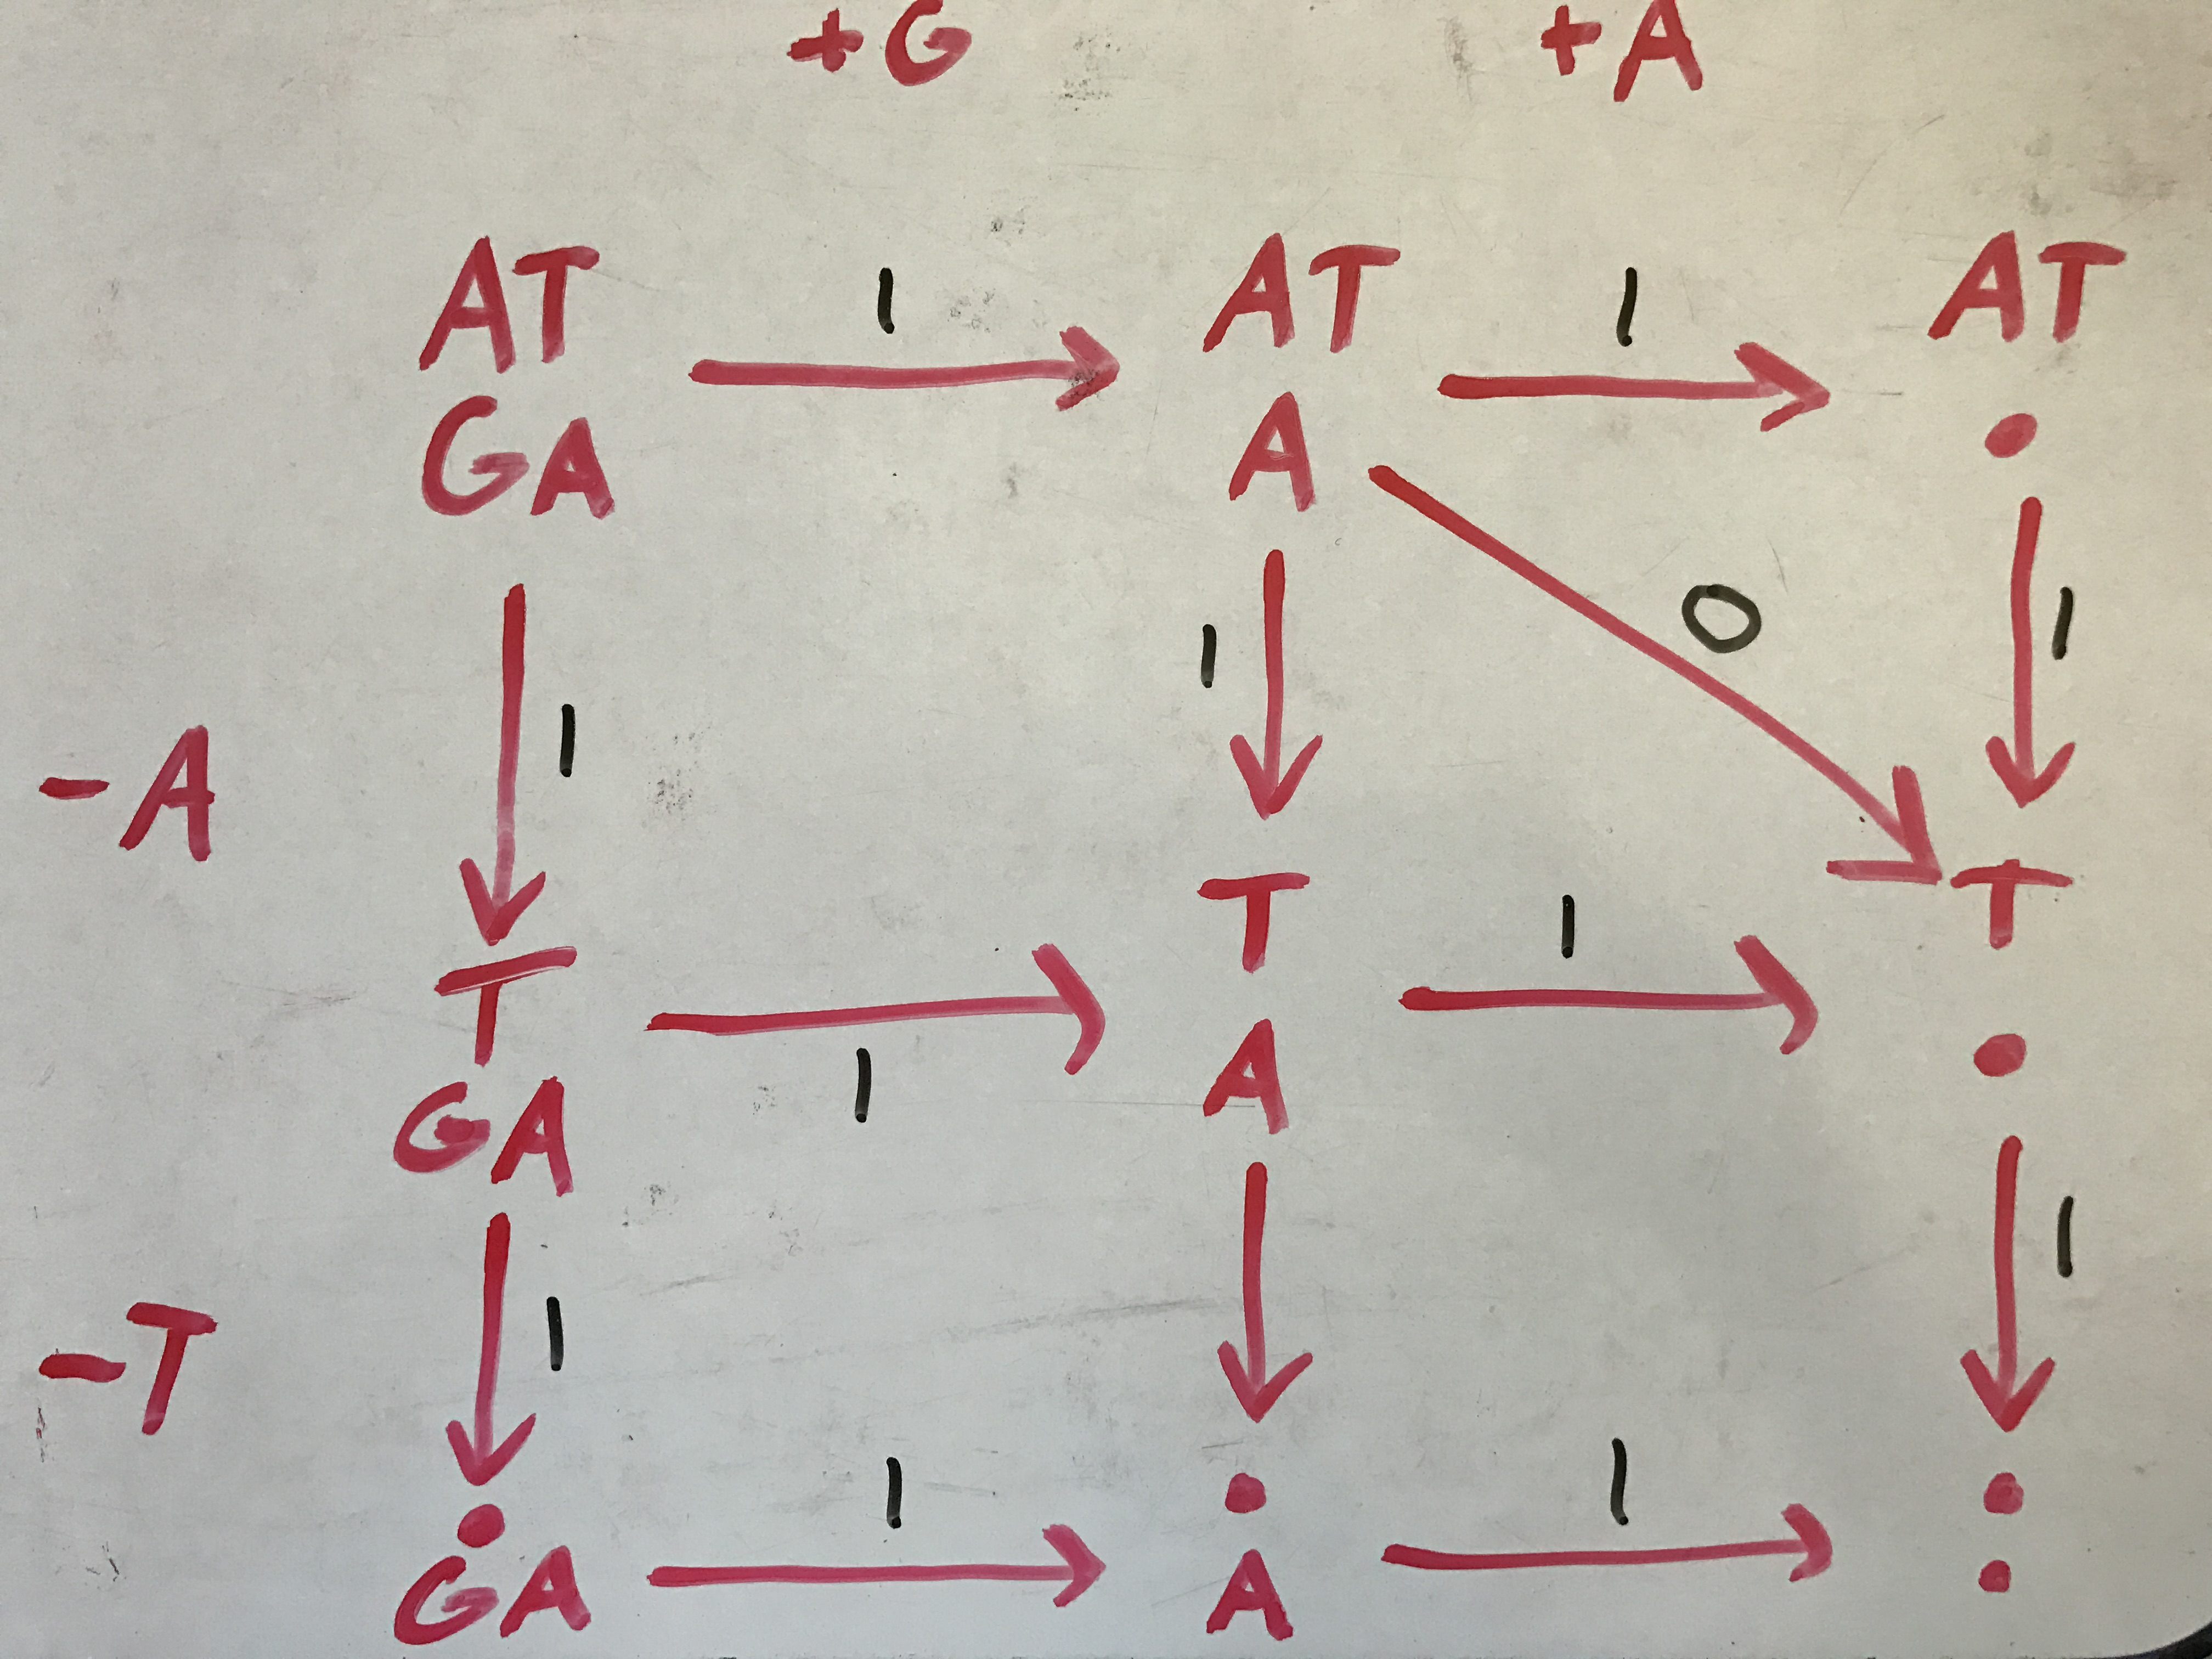
\includegraphics[scale=0.05]{geneGraph}

More generally, consider any similar graph with a grid layout where all edges
point downward, to the right, or diagonally down and to the right. Each edge is
labeled with a non-negative \textbf{cost}; the cost of a path is the sum of the
costs of the individual edges in the path. Describe an algorithm to find the
least expensive path from top left to bottom right. Analyze the speed of this
algorithm.

\textit{Bonus: also try analyzing how much \textbf{space}, i.e. \textbf{memory} on your computer, your algorithm takes,
though I did not discuss this in class. If the grid has $n \times m$ vertices,
can you make your dynamic programming solution take less than $O(n*m)$ space?}

\medskip
\textbf{Problem 3: Longest common subsequence}

A common subsequence of two strings is a list of letters that
appears in order in both strings, with any number of intervening other letters. For
example, ``GCAG'' is a \textit{longest} common subsequence of ``AGCGTAG'' and ``GTCAGC''
because it appears in both, and there is no longer one that does: ``aGCgtAG'' and ``GtCAGc''.
Describe an algorithm that finds a longest common subsequence of two strings.

\end{document}
